% Created by tikzDevice version 0.12.6 on 2026-09-15 23:29:06
% !TEX encoding = UTF-8 Unicode
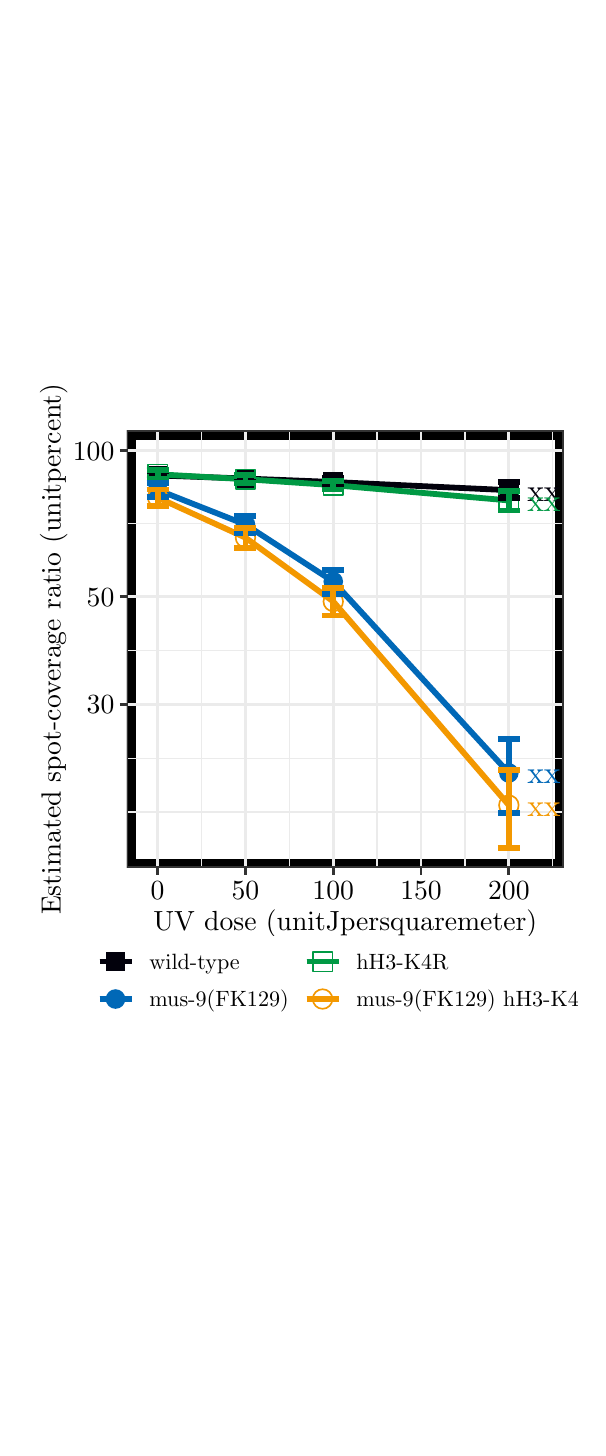
\begin{tikzpicture}[x=1pt,y=1pt]
\definecolor{fillColor}{RGB}{255,255,255}
\path[use as bounding box,fill=fillColor,fill opacity=0.00] (0,0) rectangle (198.74,505.89);
\begin{scope}
\path[clip] (  0.00,140.62) rectangle (198.74,365.27);
\definecolor{drawColor}{RGB}{255,255,255}
\definecolor{fillColor}{RGB}{255,255,255}

\path[draw=drawColor,line width= 1.0pt,line join=round,line cap=round,fill=fillColor] ( -0.00,140.62) rectangle (198.74,365.27);
\end{scope}
\begin{scope}
\path[clip] ( 35.83,202.35) rectangle (193.74,360.27);
\definecolor{drawColor}{RGB}{0,0,0}
\definecolor{fillColor}{RGB}{255,255,255}

\path[draw=drawColor,line width= 6.4pt,line join=round,line cap=round,fill=fillColor] ( 35.83,202.35) rectangle (193.74,360.27);
\definecolor{drawColor}{gray}{0.92}

\path[draw=drawColor,line width= 0.5pt,line join=round] ( 35.83,222.42) --
	(193.74,222.42);

\path[draw=drawColor,line width= 0.5pt,line join=round] ( 35.83,241.89) --
	(193.74,241.89);

\path[draw=drawColor,line width= 0.5pt,line join=round] ( 35.83,280.81) --
	(193.74,280.81);

\path[draw=drawColor,line width= 0.5pt,line join=round] ( 35.83,326.68) --
	(193.74,326.68);

\path[draw=drawColor,line width= 0.5pt,line join=round] ( 62.83,202.35) --
	( 62.83,360.27);

\path[draw=drawColor,line width= 0.5pt,line join=round] ( 94.56,202.35) --
	( 94.56,360.27);

\path[draw=drawColor,line width= 0.5pt,line join=round] (126.29,202.35) --
	(126.29,360.27);

\path[draw=drawColor,line width= 0.5pt,line join=round] (158.01,202.35) --
	(158.01,360.27);

\path[draw=drawColor,line width= 0.5pt,line join=round] (189.74,202.35) --
	(189.74,360.27);

\path[draw=drawColor,line width= 1.0pt,line join=round] ( 35.83,261.35) --
	(193.74,261.35);

\path[draw=drawColor,line width= 1.0pt,line join=round] ( 35.83,300.27) --
	(193.74,300.27);

\path[draw=drawColor,line width= 1.0pt,line join=round] ( 35.83,353.09) --
	(193.74,353.09);

\path[draw=drawColor,line width= 1.0pt,line join=round] ( 46.97,202.35) --
	( 46.97,360.27);

\path[draw=drawColor,line width= 1.0pt,line join=round] ( 78.70,202.35) --
	( 78.70,360.27);

\path[draw=drawColor,line width= 1.0pt,line join=round] (110.42,202.35) --
	(110.42,360.27);

\path[draw=drawColor,line width= 1.0pt,line join=round] (142.15,202.35) --
	(142.15,360.27);

\path[draw=drawColor,line width= 1.0pt,line join=round] (173.87,202.35) --
	(173.87,360.27);
\definecolor{drawColor}{RGB}{2,1,12}

\path[draw=drawColor,line width= 2.1pt,line join=round] ( 46.97,344.09) --
	( 78.70,342.96) --
	(110.42,341.71) --
	(173.87,338.76);
\definecolor{drawColor}{RGB}{0,153,68}

\path[draw=drawColor,line width= 2.1pt,line join=round] ( 46.97,344.51) --
	( 78.70,342.72) --
	(110.42,340.58) --
	(173.87,335.05);
\definecolor{drawColor}{RGB}{0,104,183}

\path[draw=drawColor,line width= 2.1pt,line join=round] ( 46.97,338.86) --
	( 78.70,326.34) --
	(110.42,305.75) --
	(173.87,236.57);
\definecolor{drawColor}{RGB}{243,152,0}

\path[draw=drawColor,line width= 2.1pt,line join=round] ( 46.97,336.08) --
	( 78.70,321.60) --
	(110.42,298.53) --
	(173.87,224.93);
\definecolor{fillColor}{RGB}{2,1,12}

\path[fill=fillColor] ( 43.43,340.55) --
	( 50.51,340.55) --
	( 50.51,347.62) --
	( 43.43,347.62) --
	cycle;

\path[fill=fillColor] ( 75.16,339.43) --
	( 82.23,339.43) --
	( 82.23,346.50) --
	( 75.16,346.50) --
	cycle;

\path[fill=fillColor] (106.89,338.17) --
	(113.96,338.17) --
	(113.96,345.25) --
	(106.89,345.25) --
	cycle;

\path[fill=fillColor] (170.34,335.23) --
	(177.41,335.23) --
	(177.41,342.30) --
	(170.34,342.30) --
	cycle;
\definecolor{drawColor}{RGB}{0,153,68}

\path[draw=drawColor,line width= 0.6pt,line join=round,line cap=round] ( 43.43,340.98) rectangle ( 50.51,348.05);

\path[draw=drawColor,line width= 0.6pt,line join=round,line cap=round] ( 75.16,339.18) rectangle ( 82.23,346.26);

\path[draw=drawColor,line width= 0.6pt,line join=round,line cap=round] (106.89,337.05) rectangle (113.96,344.12);

\path[draw=drawColor,line width= 0.6pt,line join=round,line cap=round] (170.34,331.51) rectangle (177.41,338.59);
\definecolor{fillColor}{RGB}{0,104,183}

\path[fill=fillColor] ( 46.97,338.86) circle (  3.54);

\path[fill=fillColor] ( 78.70,326.34) circle (  3.54);

\path[fill=fillColor] (110.42,305.75) circle (  3.54);

\path[fill=fillColor] (173.87,236.57) circle (  3.54);
\definecolor{drawColor}{RGB}{243,152,0}

\path[draw=drawColor,line width= 0.6pt,line join=round,line cap=round] ( 46.97,336.08) circle (  3.54);

\path[draw=drawColor,line width= 0.6pt,line join=round,line cap=round] ( 78.70,321.60) circle (  3.54);

\path[draw=drawColor,line width= 0.6pt,line join=round,line cap=round] (110.42,298.53) circle (  3.54);

\path[draw=drawColor,line width= 0.6pt,line join=round,line cap=round] (173.87,224.93) circle (  3.54);
\definecolor{drawColor}{RGB}{2,1,12}

\path[draw=drawColor,line width= 2.1pt,line join=round] ( 43.01,345.68) --
	( 50.94,345.68);

\path[draw=drawColor,line width= 2.1pt,line join=round] ( 46.97,345.68) --
	( 46.97,342.46);

\path[draw=drawColor,line width= 2.1pt,line join=round] ( 43.01,342.46) --
	( 50.94,342.46);

\path[draw=drawColor,line width= 2.1pt,line join=round] ( 74.73,344.32) --
	( 82.66,344.32);

\path[draw=drawColor,line width= 2.1pt,line join=round] ( 78.70,344.32) --
	( 78.70,341.59);

\path[draw=drawColor,line width= 2.1pt,line join=round] ( 74.73,341.59) --
	( 82.66,341.59);

\path[draw=drawColor,line width= 2.1pt,line join=round] (106.46,343.11) --
	(114.39,343.11);

\path[draw=drawColor,line width= 2.1pt,line join=round] (110.42,343.11) --
	(110.42,340.29);

\path[draw=drawColor,line width= 2.1pt,line join=round] (106.46,340.29) --
	(114.39,340.29);

\path[draw=drawColor,line width= 2.1pt,line join=round] (169.91,341.59) --
	(177.84,341.59);

\path[draw=drawColor,line width= 2.1pt,line join=round] (173.87,341.59) --
	(173.87,335.83);

\path[draw=drawColor,line width= 2.1pt,line join=round] (169.91,335.83) --
	(177.84,335.83);
\definecolor{drawColor}{RGB}{0,153,68}

\path[draw=drawColor,line width= 2.1pt,line join=round] ( 43.01,346.03) --
	( 50.94,346.03);

\path[draw=drawColor,line width= 2.1pt,line join=round] ( 46.97,346.03) --
	( 46.97,342.96);

\path[draw=drawColor,line width= 2.1pt,line join=round] ( 43.01,342.96) --
	( 50.94,342.96);

\path[draw=drawColor,line width= 2.1pt,line join=round] ( 74.73,344.10) --
	( 82.66,344.10);

\path[draw=drawColor,line width= 2.1pt,line join=round] ( 78.70,344.10) --
	( 78.70,341.32);

\path[draw=drawColor,line width= 2.1pt,line join=round] ( 74.73,341.32) --
	( 82.66,341.32);

\path[draw=drawColor,line width= 2.1pt,line join=round] (106.46,342.10) --
	(114.39,342.10);

\path[draw=drawColor,line width= 2.1pt,line join=round] (110.42,342.10) --
	(110.42,339.03);

\path[draw=drawColor,line width= 2.1pt,line join=round] (106.46,339.03) --
	(114.39,339.03);

\path[draw=drawColor,line width= 2.1pt,line join=round] (169.91,338.54) --
	(177.84,338.54);

\path[draw=drawColor,line width= 2.1pt,line join=round] (173.87,338.54) --
	(173.87,331.40);

\path[draw=drawColor,line width= 2.1pt,line join=round] (169.91,331.40) --
	(177.84,331.40);
\definecolor{drawColor}{RGB}{0,104,183}

\path[draw=drawColor,line width= 2.1pt,line join=round] ( 43.01,341.30) --
	( 50.94,341.30);

\path[draw=drawColor,line width= 2.1pt,line join=round] ( 46.97,341.30) --
	( 46.97,336.35);

\path[draw=drawColor,line width= 2.1pt,line join=round] ( 43.01,336.35) --
	( 50.94,336.35);

\path[draw=drawColor,line width= 2.1pt,line join=round] ( 74.73,329.38) --
	( 82.66,329.38);

\path[draw=drawColor,line width= 2.1pt,line join=round] ( 78.70,329.38) --
	( 78.70,323.18);

\path[draw=drawColor,line width= 2.1pt,line join=round] ( 74.73,323.18) --
	( 82.66,323.18);

\path[draw=drawColor,line width= 2.1pt,line join=round] (106.46,309.96) --
	(114.39,309.96);

\path[draw=drawColor,line width= 2.1pt,line join=round] (110.42,309.96) --
	(110.42,301.29);

\path[draw=drawColor,line width= 2.1pt,line join=round] (106.46,301.29) --
	(114.39,301.29);

\path[draw=drawColor,line width= 2.1pt,line join=round] (169.91,248.72) --
	(177.84,248.72);

\path[draw=drawColor,line width= 2.1pt,line join=round] (173.87,248.72) --
	(173.87,222.13);

\path[draw=drawColor,line width= 2.1pt,line join=round] (169.91,222.13) --
	(177.84,222.13);
\definecolor{drawColor}{RGB}{243,152,0}

\path[draw=drawColor,line width= 2.1pt,line join=round] ( 43.01,338.99) --
	( 50.94,338.99);

\path[draw=drawColor,line width= 2.1pt,line join=round] ( 46.97,338.99) --
	( 46.97,333.05);

\path[draw=drawColor,line width= 2.1pt,line join=round] ( 43.01,333.05) --
	( 50.94,333.05);

\path[draw=drawColor,line width= 2.1pt,line join=round] ( 74.73,325.14) --
	( 82.66,325.14);

\path[draw=drawColor,line width= 2.1pt,line join=round] ( 78.70,325.14) --
	( 78.70,317.89);

\path[draw=drawColor,line width= 2.1pt,line join=round] ( 74.73,317.89) --
	( 82.66,317.89);

\path[draw=drawColor,line width= 2.1pt,line join=round] (106.46,303.27) --
	(114.39,303.27);

\path[draw=drawColor,line width= 2.1pt,line join=round] (110.42,303.27) --
	(110.42,293.47);

\path[draw=drawColor,line width= 2.1pt,line join=round] (106.46,293.47) --
	(114.39,293.47);

\path[draw=drawColor,line width= 2.1pt,line join=round] (169.91,237.73) --
	(177.84,237.73);

\path[draw=drawColor,line width= 2.1pt,line join=round] (173.87,237.73) --
	(173.87,209.53);

\path[draw=drawColor,line width= 2.1pt,line join=round] (169.91,209.53) --
	(177.84,209.53);
\definecolor{drawColor}{RGB}{2,1,12}

\node[text=drawColor,anchor=base,inner sep=0pt, outer sep=0pt, scale=  1.14] at (186.56,334.85) {xx};
\definecolor{drawColor}{RGB}{0,153,68}

\node[text=drawColor,anchor=base,inner sep=0pt, outer sep=0pt, scale=  1.14] at (186.56,331.13) {xx};
\definecolor{drawColor}{RGB}{0,104,183}

\node[text=drawColor,anchor=base,inner sep=0pt, outer sep=0pt, scale=  1.14] at (186.56,232.66) {xx};
\definecolor{drawColor}{RGB}{243,152,0}

\node[text=drawColor,anchor=base,inner sep=0pt, outer sep=0pt, scale=  1.14] at (186.56,221.01) {xx};
\definecolor{drawColor}{gray}{0.20}

\path[draw=drawColor,line width= 1.0pt,line join=round,line cap=round] ( 35.83,202.35) rectangle (193.74,360.27);
\end{scope}
\begin{scope}
\path[clip] (  0.00,  0.00) rectangle (198.74,505.89);
\definecolor{drawColor}{RGB}{0,0,0}

\node[text=drawColor,anchor=base east,inner sep=0pt, outer sep=0pt, scale=  1.00] at ( 31.33,257.91) {30};

\node[text=drawColor,anchor=base east,inner sep=0pt, outer sep=0pt, scale=  1.00] at ( 31.33,296.83) {50};

\node[text=drawColor,anchor=base east,inner sep=0pt, outer sep=0pt, scale=  1.00] at ( 31.33,349.65) {100};
\end{scope}
\begin{scope}
\path[clip] (  0.00,  0.00) rectangle (198.74,505.89);
\definecolor{drawColor}{gray}{0.20}

\path[draw=drawColor,line width= 1.0pt,line join=round] ( 33.33,261.35) --
	( 35.83,261.35);

\path[draw=drawColor,line width= 1.0pt,line join=round] ( 33.33,300.27) --
	( 35.83,300.27);

\path[draw=drawColor,line width= 1.0pt,line join=round] ( 33.33,353.09) --
	( 35.83,353.09);
\end{scope}
\begin{scope}
\path[clip] (  0.00,  0.00) rectangle (198.74,505.89);
\definecolor{drawColor}{gray}{0.20}

\path[draw=drawColor,line width= 1.0pt,line join=round] ( 46.97,199.85) --
	( 46.97,202.35);

\path[draw=drawColor,line width= 1.0pt,line join=round] ( 78.70,199.85) --
	( 78.70,202.35);

\path[draw=drawColor,line width= 1.0pt,line join=round] (110.42,199.85) --
	(110.42,202.35);

\path[draw=drawColor,line width= 1.0pt,line join=round] (142.15,199.85) --
	(142.15,202.35);

\path[draw=drawColor,line width= 1.0pt,line join=round] (173.87,199.85) --
	(173.87,202.35);
\end{scope}
\begin{scope}
\path[clip] (  0.00,  0.00) rectangle (198.74,505.89);
\definecolor{drawColor}{RGB}{0,0,0}

\node[text=drawColor,anchor=base,inner sep=0pt, outer sep=0pt, scale=  1.00] at ( 46.97,190.97) {0};

\node[text=drawColor,anchor=base,inner sep=0pt, outer sep=0pt, scale=  1.00] at ( 78.70,190.97) {50};

\node[text=drawColor,anchor=base,inner sep=0pt, outer sep=0pt, scale=  1.00] at (110.42,190.97) {100};

\node[text=drawColor,anchor=base,inner sep=0pt, outer sep=0pt, scale=  1.00] at (142.15,190.97) {150};

\node[text=drawColor,anchor=base,inner sep=0pt, outer sep=0pt, scale=  1.00] at (173.87,190.97) {200};
\end{scope}
\begin{scope}
\path[clip] (  0.00,  0.00) rectangle (198.74,505.89);
\definecolor{drawColor}{RGB}{0,0,0}

\node[text=drawColor,anchor=base,inner sep=0pt, outer sep=0pt, scale=  1.00] at (114.79,179.64) {UV dose (unit{Jpersquaremeter})};
\end{scope}
\begin{scope}
\path[clip] (  0.00,  0.00) rectangle (198.74,505.89);
\definecolor{drawColor}{RGB}{0,0,0}

\node[text=drawColor,rotate= 90.00,anchor=base,inner sep=0pt, outer sep=0pt, scale=  1.00] at ( 11.89,281.31) {Estimated spot-coverage ratio (unit{percent})};
\end{scope}
\begin{scope}
\path[clip] (  0.00,  0.00) rectangle (198.74,505.89);
\definecolor{fillColor}{RGB}{255,255,255}

\path[fill=fillColor] ( 19.53,145.62) rectangle (210.04,177.69);
\end{scope}
\begin{scope}
\path[clip] (  0.00,  0.00) rectangle (198.74,505.89);
\definecolor{drawColor}{RGB}{2,1,12}

\path[draw=drawColor,line width= 2.1pt,line join=round] ( 25.97,168.42) -- ( 37.53,168.42);
\definecolor{fillColor}{RGB}{2,1,12}

\path[fill=fillColor] ( 28.22,164.89) --
	( 35.29,164.89) --
	( 35.29,171.96) --
	( 28.22,171.96) --
	cycle;

\path[draw=drawColor,line width= 2.1pt,line join=round] ( 25.97,168.42) -- ( 37.53,168.42);
\end{scope}
\begin{scope}
\path[clip] (  0.00,  0.00) rectangle (198.74,505.89);
\definecolor{drawColor}{RGB}{0,153,68}

\path[draw=drawColor,line width= 2.1pt,line join=round] (100.79,168.42) -- (112.35,168.42);

\path[draw=drawColor,line width= 0.6pt,line join=round,line cap=round] (103.04,164.89) rectangle (110.11,171.96);

\path[draw=drawColor,line width= 2.1pt,line join=round] (100.79,168.42) -- (112.35,168.42);
\end{scope}
\begin{scope}
\path[clip] (  0.00,  0.00) rectangle (198.74,505.89);
\definecolor{drawColor}{RGB}{0,104,183}

\path[draw=drawColor,line width= 2.1pt,line join=round] ( 25.97,154.89) -- ( 37.53,154.89);
\definecolor{fillColor}{RGB}{0,104,183}

\path[fill=fillColor] ( 31.75,154.89) circle (  3.54);

\path[draw=drawColor,line width= 2.1pt,line join=round] ( 25.97,154.89) -- ( 37.53,154.89);
\end{scope}
\begin{scope}
\path[clip] (  0.00,  0.00) rectangle (198.74,505.89);
\definecolor{drawColor}{RGB}{243,152,0}

\path[draw=drawColor,line width= 2.1pt,line join=round] (100.79,154.89) -- (112.35,154.89);

\path[draw=drawColor,line width= 0.6pt,line join=round,line cap=round] (106.57,154.89) circle (  3.54);

\path[draw=drawColor,line width= 2.1pt,line join=round] (100.79,154.89) -- (112.35,154.89);
\end{scope}
\begin{scope}
\path[clip] (  0.00,  0.00) rectangle (198.74,505.89);
\definecolor{drawColor}{RGB}{0,0,0}

\node[text=drawColor,anchor=base west,inner sep=0pt, outer sep=0pt, scale=  0.80] at ( 43.98,165.67) {wild-type};
\end{scope}
\begin{scope}
\path[clip] (  0.00,  0.00) rectangle (198.74,505.89);
\definecolor{drawColor}{RGB}{0,0,0}

\node[text=drawColor,anchor=base west,inner sep=0pt, outer sep=0pt, scale=  0.80] at (118.80,165.67) {hH3-K4R};
\end{scope}
\begin{scope}
\path[clip] (  0.00,  0.00) rectangle (198.74,505.89);
\definecolor{drawColor}{RGB}{0,0,0}

\node[text=drawColor,anchor=base west,inner sep=0pt, outer sep=0pt, scale=  0.80] at ( 43.98,152.13) {mus-9(FK129)};
\end{scope}
\begin{scope}
\path[clip] (  0.00,  0.00) rectangle (198.74,505.89);
\definecolor{drawColor}{RGB}{0,0,0}

\node[text=drawColor,anchor=base west,inner sep=0pt, outer sep=0pt, scale=  0.80] at (118.80,152.13) {mus-9(FK129) hH3-K4R};
\end{scope}
\end{tikzpicture}
